\documentclass[../main.tex]{subfiles}

\begin{document}

\subsection{Utformning}

Med hjälp av det givna strukturdiagrammet,\\

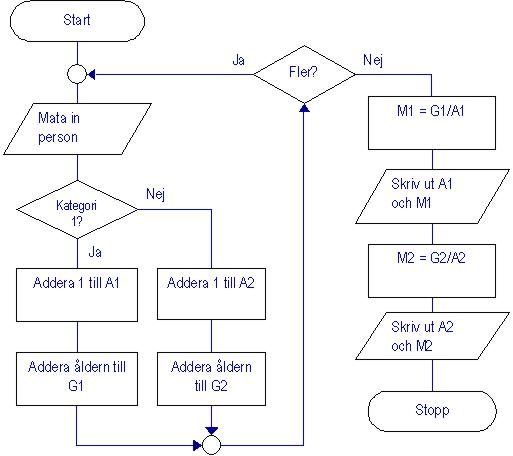
\includegraphics[width=11cm, height=10cm]{Projekt/Genomsnitt/figs/strukturdiagram.jpg}
\\
underlättar vi konstruktionens detaljerade nivåer, genom att bryta ned diagrammet i sektioner,

\begin{tcolorbox}[colback=gray!5!white,colframe=black!75!black]

\begin{enumerate}

    \item \textbf{Indata}. Här definieras vilken information vi behöver av användaren för att kunna beräkna och få de resultat vi är ute efter.
    
    \item \textbf{Selektion}. Här beskrivs hanterandet av sorteringen av de två grupperna. 
    
    \item \textbf{Iteration}. Här beskrivs upprepningen av ovanstående sektioner.
    Vill användaren lägga till fler personer i populationen? Om ja upprepa 1 och 2, annars fortsätt med 4.
    
    \item \textbf{Kalkyl}. Hur gruppernas ålder adderas och divideras för att få genomsnittsåldern i respektive grupp.
    
    \item \textbf{Utdata}. Presentationen av resultaten till användaren.
    
\end{enumerate}

\end{tcolorbox}

\newpage

\end{document}